 \documentclass{report}
 
\usepackage[utf8]{inputenc} 
\usepackage[T1]{fontenc}      
\usepackage[top=2.0cm, bottom=3cm, left=3.0cm, right=3.0cm]{geometry}
\usepackage{graphicx}
\usepackage{wrapfig}
\usepackage{amsmath,esint }
\usepackage{amssymb}
\graphicspath{{figures/}{../figures}}

\newcommand*\dif{\mathop{}\!\mathrm{d}}
\newcommand*\diver{\mathop{}\!\mathrm{div}}
\newcommand*\grad{\mathop{}\!\mathrm{grad}}

\begin{document}

\section*{Onde cylindrique}

A partir d'un fil source d'axe $Oz$, est émise une dans le vide une onde dont le champ est donné en coordonnées cylindriques par :
\begin{align*}
	\vec{E}=E(r)e^{i(\omega t-kr)}\vec{e}_z
\end{align*}

\begin{itemize}

	\item[$\circ$] Trouver le champ magnétique correspondant. Commenter.
	
	\item[$\circ$] Déterminer le vecteur de Poynting instantané $\vec{\Pi}$, puis sa moyenne temporelle.
	
	\item[$\circ$] Quelle est la puissance moyenne rayonnée à travers un cylindre d'axe $Oz$, de rayon $r$ et de hauteur $h$ ? En déduire la dépendance $E(r)$. 
	
	\item[$\circ$] Quelle est l'expression de $\vec{B}$ à grande distance ? Commenter.
	
\end{itemize}

\newpage

\section*{Répartition de l'énergie volumique dans un plasma}

Un plasma est traversé par une onde électromagnétique plane progressive harmonique se propageant suivant les $z$ croissants, dont le champ électrique est polarisé, rectilignement selon $\vec{e}_x$. On suppose que sa pulsation $\omega$ est supérieure à la pulsation plasma $\omega_p=\sqrt{\frac{n_0e^2}{\varepsilon_0m_e}}$, où $n_0$ est la densité volumique d'électrons et $m_e$ la masse de l'électron.

\begin{itemize}

	\item[$\bigotimes$] Donner l'expression du champ électrique, en notant $E_0$ son amplitude.
	
	\item[$\bigotimes$] Rappeler l'expression de $k^2$ en fonction de $\omega$ et $\omega_P$. Que se serait-il passé si $\omega<\omega_P$ ? 
	
	\item[$\bigotimes$] Calculer l'expression du champ magnétique $\vec{B}(z,t)$. 
	
	\item[$\bigotimes$] Donner l'expression des énergies électriques et magnétiques moyennées au cours du temps, $\left\langle u_e\right\rangle $ et $\left\langle u_m\right\rangle $ ?
	
	\item[$\bigotimes$] Pourquoi dit-on qu'il y a équipartition de l'énergie dans le vide ? Est-ce le cas dans le plasma ?
	
	\item[$\bigotimes$] Déterminer l'énergie cinétique moyenne des électrons $\left\langle e_c \right\rangle$. Conclure.
	
\end{itemize}

\newpage

\section*{Réflexion d'une onde polarisée}

Une onde plane électromagnétique se propageant dans le vide dans le demi-espace $x<0$ vers les $x$ croissants tombe en incidence normale, en $x=0$, sur un métal remplissant le demi espace $x>0$ à partir du plan $yOz$. Le métal est supposé parfait.

\begin{itemize}

	\item[$\circlearrowright$] Qu'est-ce qu'un métal parfait ? En déduire les conséquences sur l'onde transmise. 

\end{itemize}

Le champ électrique de l'onde incidente s'écrit :
\begin{align*}
	\vec{E}_i=E_0\cos(\omega t -kx)\vec{e}_y+E_0\sin(\omega t -kx)\vec{e}_z
\end{align*}

\begin{itemize}

	\item[$\circlearrowright$] Quelle est la polarisation de cette onde? Justifier. 
	
	\item[$\circlearrowright$] En déduire le champ électrique réfléchi $\vec{E}_r$. On rappelle qu'à l'interface en $x=0$, la composante tangentielle du champ électrique est continue.
	
	\item[$\circlearrowright$] Quelle est la polarisation de l'onde réfléchie ? 
	
	\item[$\circlearrowright$] Déterminer l'expression du champ électrique total $\vec{E}$.
	
	\item[$\circlearrowright$] Donner l'expression du champ magnétique incident $\vec{B}_i$ et réfléchi $\vec{B}_r$. Le champ magnétique est-il continu en $x=0$ ? Expliquer. 

\end{itemize}

\newpage

\section*{\textit{Correction - Réflexion d'une onde polarisée}}

\begin{itemize}

	\item[$\circlearrowright$] Conductivité infinie, le champ électromagnétique ne pénètre pas dans le métal, les courants sont uniquement en surface.

\end{itemize}

Le champ électrique de l'onde incidente s'écrit :
\begin{align*}
	\vec{E}_i=E_{0_i}\cos(\omega t -kx)\vec{e}_y+E_{0_i}\sin(\omega t -kx)\vec{e}_z
\end{align*}

\begin{itemize}

	\item[$\circlearrowright$] C'est une onde polarisée circulairement : la pointe du vecteur $\vec{E}$ décrit à une position fixée un cercle au cours du temps. Dans ce cas, il tourne dans le sens trigonométrique lorsqu'on regarde l'onde arriver vers nous. 
	
	\item[$\circlearrowright$] Comme le champ électrique est continu (car uniquement tangentiel), on a en $x=0$ :
	\begin{align*}
		\vec{E}_i(x=0)+\vec{E}_r(x=0)=\vec{0}
	\end{align*}
	Donc :
	\begin{align*}
		\vec{E}_r(x=0)=-E_{0_i}\cos(\omega t)\vec{e}_y-E_0\sin(\omega t)\vec{e}_z
	\end{align*}	
	Comme l'onde réfléchie se propage suivant les $x$ décroissant, son expression est alors nécessairement de la forme :
	\begin{align*}
		\vec{E}_r=-E_{0_i}\cos(\omega t+kx)\vec{e}_y-E_{0_i}\sin(\omega t +kx)\vec{e}_z
	\end{align*}	
	
	\item[$\circlearrowright$] Elle est aussi polarisée circulairement mais elle tourne dans l'autre sens : elle tourne dans le même sens que l'onde incidente, mais se propage dans la direction opposée. Elle tourne donc dans le sens horaire lorsqu'on regarde l'onde arriver vers nous. 
	
	\item[$\circlearrowright$] On additionne le champ incident et réfléchi : 
	\begin{align*}
		\vec{E}=2E_{0_i}\sin(\omega t)\sin(kx)\vec{e}_y-2E_{0_i}\sin(kx)\cos(\omega t)\vec{e}_z
	\end{align*}
	\item[$\circlearrowright$] On utilise la relation de structure, avec $\vec{k}_i=\omega/c\vec{e}_x$ :
	\begin{align*}
		\vec{B}_i=&\frac{\vec{k}_i\wedge\vec{E}_i}{\omega} \\
		=&\frac{E_{0_i}}{c}\cos(\omega t -kx)\vec{e}_y+\frac{E_{0_i}}{c}\sin(\omega t -kx)\vec{e}_z
	\end{align*}
	Même chose pour le champ réfléchi, avec $\vec{k}_r=-\omega/c\vec{e}_x$ :
	\begin{align*}
		\vec{B}_r=&\frac{\vec{k}_r\wedge\vec{E}_r}{\omega} \\
		=&\frac{E_{0_i}}{c}\cos(\omega t +kx)\vec{e}_y+\frac{E_{0_i}}{c}\sin(\omega t +kx)\vec{e}_z
	\end{align*}
	On remarque qu'en $x=0$, on a :
	\begin{align*}
		\vec{B}(x=0)=\frac{2E_{0_i}}{c}\cos(\omega t)\vec{e}_y+\frac{2E_{0_i}}{c}\sin(\omega t)\vec{e}_z
	\end{align*}
	La composante transverse du champ magnétique n'est pas systématiquement continue : dans le cas de la présence de courants surfaciques, il ne l'est pas, ce qui est le cas ici.

\end{itemize}

\newpage

\section*{Réflexion d'une onde électromagnétique sur des plans métalliques en incidence oblique $\bullet\bullet\circ$}

On considère une onde plane progressive se propageant dans le vide, selon le vecteur d'onde $\vec{k}=k\cos\theta\vec{u_x}+k\sin\theta\vec{u_y}$ et à la pulsation $\omega$. Elle arrive sur un plan métallique infiniment conducteur situé sur le demi-espace $x>0$. On notera $\vec{E_i}$ et $\vec{B_i}$ respectivement le champ électrique et le champ magnétique incidents. Le champ électrique incident est polarisé rectilignement selon $Oz$ et son amplitude est $E_0$.

\begin{itemize}
		
	\item[$\heartsuit$]	Retrouver l'équation de propagation des champs électrique et magnétique. Quelle est la relation de dispersion associée ? 
	
	\item[$\heartsuit$] Expliciter les expressions des champs $\vec{E_i}$ et $\vec{B_i}$.
	
\end{itemize}

En arrivant sur l'interface, les relations de passage du champ électromagnétique imposent l'apparition d'une onde réfléchie, dont on notera $\vec{E_r}$ et $\vec{B_r}$ les champ électrique et magnétique. On supposera que $\vec{E_r}$ s'écrit sous la forme : 
\begin{align*}
	\vec{E_r}=\vec{E_0'}\exp(i\vec{k_r}\cdot\vec{r}-\omega t)
\end{align*}
avec $\vec{k_r}=-k\cos\theta\vec{u_x}+k\sin\theta\vec{u_y}$ est le vecteur d'onde de l'onde réfléchi.
\begin{itemize}
	
	\item[$\heartsuit$] Que valent les champs $\vec{E}$ et $\vec{B}$ à l'intérieur de la plaque ? Justifier.
	
	\item[$\heartsuit$] Déterminer $\vec{E_0'}$. On rappelle que la composante tangentielle du champ électrique est toujours continue, même sur une interface.
	
	\item[$\heartsuit$] En déduire l'expression du champ magnétique réfléchi, $\vec{B_r}$.
	
	\item[$\heartsuit$] Quelle est alors l'expression du champ électrique $\vec{E}$ résultant pour $x<0$ ? De quel type d'onde s'agit-il ?
	
	\item[$\heartsuit$] 	On place une seconde plaque métallique en $x=-L$. Montrer que la présence de la seconde plaque impose une discrétisation du spectre, c'est-à-dire que seules des fréquences $\omega$ discrètes peuvent se propager pour un angle $\theta$ donné. Tracer les valeurs prises par $\omega$ en fonction de $\theta$. 
	\item[$\heartsuit$] Quelle est la valeur minimale que peut prendre $\omega$ ? Justifier. 
	
	\item[$\heartsuit$] Démontrer que $k_y=\vec{k}\cdot\vec{u_y}$ vérifie l'équation dite de dispersion des modes d'une onde transverse électrique : 
	\begin{equation}
		k_y^2=\frac{\omega^2}{c^2}-\left(\frac{n\pi}{a} \right)^2 
	\end{equation}
	
	\item[$\heartsuit$] Quel est le courant surfacique à la surface de la plaque ?
	
	\item[$\heartsuit$] Calculer l'expression du champ magnétique résultant $\vec{B}$ entre les deux plaques et en déduire l'expression du vecteur de Poyting. Commenter. 
	
\end{itemize}

\newpage

\section*{Réflexion d'une onde électromagnétique sur des plans métalliques en incidence oblique $\bullet\bullet\bullet$}

On considère une onde plane progressive se propageant dans le vide, selon le vecteur d'onde $\vec{k}=k\cos\theta\vec{u_x}+k\sin\theta\vec{u_y}$ et à la pulsation $\omega$. Elle arrive sur un plan métallique infiniment conducteur situé sur le demi-espace $x>0$. On notera $\vec{E_i}$ et $\vec{B_i}$ respectivement le champ électrique et le champ magnétique incidents. Le champ électrique incident est polarisé rectilignement selon $Oz$ et son amplitude est $E_0$.

\begin{itemize}
		
	\item[$\heartsuit$]	Retrouver l'équation de propagation des champs électrique et magnétique. Quelle est la relation de dispersion associée ? 
	
	\item[$\heartsuit$] Expliciter les expressions des champs $\vec{E_i}$ et $\vec{B_i}$.
	
\end{itemize}

En arrivant sur l'interface, les relations de passage du champ électromagnétique imposent l'apparition d'une onde réfléchie, dont on notera $\vec{E_r}$ et $\vec{B_r}$ les champ électrique et magnétique. On supposera que $\vec{E_r}$ s'écrit sous la forme : 
\begin{align*}
	\vec{E_r}=\vec{E_0'}\exp(i\vec{k_r}\cdot\vec{r}-\omega t)
\end{align*}
avec $\vec{k_r}=k_r\cos\theta_r\vec{u_x}+k_r\sin\theta_r\vec{u_y}$, où $\theta_r$ est l'angle de réflexion de l'onde, à priori différent de $\theta$.
\begin{itemize}
	
	\item[$\heartsuit$] Que valent les champs $\vec{E}$ et $\vec{B}$ à l'intérieur de la plaque ? Justifier.
	
	\item[$\heartsuit$] En utilisant les relations de passage, déterminer $\vec{E_0'}$ puis $\theta_r$ pour en déduire l'expression de $\vec{E_r}$ en fonction de $E_0$, $k$, $\omega$ et $\theta$. Quel est le lien avec la loi de Descartes sur la réflexion ?
	
	\item[$\heartsuit$] En déduire l'expression du champ magnétique réfléchi, $\vec{B_r}$.
	
	\item[$\heartsuit$] Quelle est alors l'expression du champ électrique $\vec{E}$ résultant pour $x<0$ ? De quel type d'onde s'agit-il ?
	
	\item[$\heartsuit$] 	On place une seconde plaque métallique en $x=-L$. Montrer que la présence de la seconde plaque impose une discrétisation du spectre, c'est-à-dire que seules des fréquences $\omega$ discrètes peuvent se propager pour un angle $\theta$ donné. Tracer les valeurs prises par $\omega$ en fonction de $\theta$. 
	\item[$\heartsuit$] Quelle est la valeur minimale que peut prendre $\omega$ ? Justifier. 
	
	\item[$\heartsuit$] Démontrer que $k_y=\vec{k}\cdot\vec{u_y}$ vérifie l'équation dite de dispersion des modes d'une onde transverse électrique : 
	\begin{equation}
		k_y^2=\frac{\omega^2}{c^2}-\left(\frac{n\pi}{a} \right)^2 
	\end{equation}
	
	\item[$\heartsuit$] Quel est le courant surfacique à la surface de la plaque ?
	
	\item[$\heartsuit$] Calculer l'expression du champ magnétique résultant $\vec{B}$ entre les deux plaques et en déduire l'expression du vecteur de Poyting. Commenter. 
	
\end{itemize}

\newpage

\section*{Propagation d'une onde radio dans un plasma en présence d'un champ magnétique longitudinal (à simplifier)}

Le plasma ionosphérique est assimilé à un milieu conducteur ionisé de temps de relaxation infini, c'est-à-dire qu'il n'y a pas de collisions. Le plasma est supposé neutre et sa densité électronique est $n_0$. On tient compte ici du champ magnétostatique terrestre désigné par $\vec{B}_{ext}=B_{ext}\vec{u_z}$, dirigé selon la direction de propagation $Oz$ d'une OPPM électromagnétique de pulsation $\omega$, dont le champ est représenté par :
\begin{align*}
	(\vec{E},\vec{B})=(\vec{E}_0,\vec{B}_0)\exp[j(\omega t-kz)]
\end{align*}
On note $\omega_p=\sqrt{n_0e^2/m\varepsilon_0}$ la pulsation de plasma du milieu et $\omega_c=eB_{ext}/m$ la pulsation cyclotron. 

\begin{itemize}
	
	\item[$\spadesuit$] Montrer que le champ magnétique terrestre intervient dans la conduction électrique du milieu, qui peut être représenté par une relation linéaire :
	\begin{align*}
		\vec{j}=\left[\gamma \right] \vec{E}
	\end{align*}
	où $\left[\gamma \right]$ est une matrice de conductivité complexe, à exprimer en fonction de $\omega$, $\omega_c$ et $\omega_p$.
	
\end{itemize}

Une onde est polarisée circulairement lorsque les composantes transverses sont déphasées de $\pm\pi/2$, c'est-à-dire dans notre cas, en notation réelle :
\begin{equation}
	\vec{E}=E_0\cos(\omega t - kz)\vec{e_x}\pm E_0\sin(\omega t - kz)\vec{e_y}
\end{equation}
Un signe "+" correspond à une onde polarisée circulairement "gauche" et le signe "-" à une onde polarisée circulaire "droite". On cherche à comprendre la propagation de ces ondes dans le plasma.

\begin{itemize}

	\item[$\spadesuit$] Pourquoi appelle t-on cette polarisation "circulaire" ? 
	
	\item[$\spadesuit$] Montrer que l'étude de la propagation des OPPM électromagnétiques peut être ramenée à celle d'ondes polarisées circulairement qui satisfont des relations de dispersion à préciser. 
	
\end{itemize}

On appelle permittivité relative d'un milieu la quantité complexe $\varepsilon_r$ que l'on peut définir ici à travers la relation $k^2=\varepsilon_r\varepsilon_0\mu_0\omega^2=\varepsilon_r\omega^2/c^2$. 

\begin{itemize}

	\item[$\spadesuit$] On note $\varepsilon_{rg}$ et $\varepsilon_{rd}$ les permittivités relatives équivalentes associées respectivement à la propagation des ondes circulaires gauche et des ondes circulaires droites, dont les graphes sont donnés ci-dessous. Donner leur expression. Préciser les domaines du spectre électromagnétique pour lesquels les ondes étudiées se propagent effectivement dans le plasma.

\end{itemize}

Une onde métrique traverse une épaisseur $L$ de plasma dans les conditions de l'étude effectuée. A l'entrée de la couche de plasma, l'onde est polarisée rectilignement.

\begin{itemize}
	
	\item[$\spadesuit$] Montrer, dans le cas général, qu'un onde polarisée rectilignement peur s'écrire comme la superposition d'une onde polarisée circulaire droite et circulaire gauche. 
	
	\item[$\spadesuit$] Justifier alors que l'effet du plasma consiste, aux hautes fréquences, en une rotation de la direction de polarisation de l'onde. Préciser la valeur de cet angle si $L=1$km et $\lambda_0=30$cm.
	
\end{itemize}

\textit{Données} : $e=1,6\cdot10^{-19}$C, $m=9,1\cdot10^{-31}$kg, $\varepsilon_0=8,85\cdot10^{-12}$F/m, $n_0=10^{12}$m$^{-3}$, $B_{ext}=5\cdot10^{-5}$T.

\newpage

\begin{figure}[h!]
\centering
  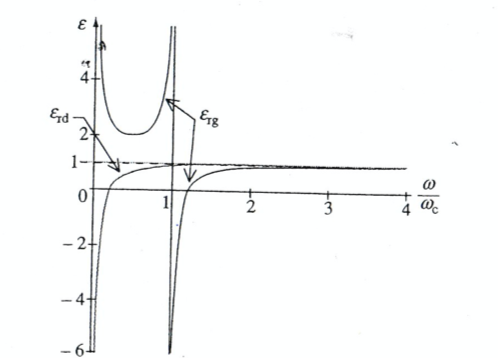
\includegraphics[width=0.6\textwidth]{permittivite1.png}
\end{figure}

\newpage

\section*{Ondes électromagnétiques dans un métal conducteur}

On s'intéresse ici à la propagation des ondes électromagnétiques dans un conducteur métallique, en fonction de leur fréquence et des caractéristiques du métal. Plus particulièrement, on souhaite savoir pourquoi un métal est réfléchissant à basse fréquence, mais transparent à partir d'une certaine fréquence.

On considère donc que le demi-espace $z>0$ est rempli d'un métal conducteur, sur lequel arrive une onde plane progressive monochromatique à la fréquence $\omega$ et dont le champ électrique est polarisé suivant $\vec{e_x}$, se propageant suivant les $z$ croissants. 

\begin{itemize}

	\item[$\diamondsuit$] Retrouver l'équation de propagation des ondes électromagnétiques dans le vide. A l'aide des données de l'énoncé, donner l'expression du champ $\vec{E}$ et du champ $\vec{B}$ pour $z<0$.

\end{itemize}

Pour décrire le métal, on adopte un modèle d'électrons libres de masse $m$, de charge $-e$ et de densité particulaire $N_0$, soumis au champ électromagnétique, et subissant des collisions en moyenne au bout d'un temps $\tau=1/\omega_c$. On modélise alors le comportement des électrons par l'équation de mouvement (aussi appelé modèle de Drude) :

\begin{equation}
	m\vec{a}=-e\vec{E}-m\frac{\vec{v}}{\tau}
	\label{eq:drude}
\end{equation}

Pour un métal très conducteur, on a $N_0\simeq10^{29}$m$^{-3}$ et $\tau\simeq10^{-14}$s.

\textbf{Revoir l'organisation des questions, l'enchainement n'es tpas limpide}

\begin{itemize}

	\item[$\diamondsuit$] En utilisant l'équation \ref{eq:drude}, définir une conductivité du métal $\gamma$ complexe, lorsqu'il est soumis à une OPPM comme proposé ci-dessus. On fera apparaître la pulsation plasma $\omega_p=\sqrt{N_0e^2/m\varepsilon_0}$. 
	
	\item[$\diamondsuit$] En utilisant les équations de Maxwell, déterminer la relation de dispersion des OPPM dans le métal. 
	
	\item[$\diamondsuit$] Comparer $\omega_c=1/\tau$ et $\omega_p$. Justifier de l'existence de 3 régimes de propagation dans le métal que nous allons étudier par la suite.

\end{itemize}

\textbf{On se place dans le cas où $\omega\ll\omega_c$.}

\begin{itemize}

	\item[$\diamondsuit$] Que devient la relation de dispersion dans ce cas-là ? Trouver les solutions possibles pour $k$. Faire apparaitre l'expression de la conductivité statique $\gamma_0$ en fonction de $\omega_p$, $\tau$ et $\varepsilon_0$.

	\item[$\diamondsuit$] Écrire l'expression du champ $\vec{E}$ dans le métal, puis celle du champ $\vec{B}$. Comment appelle t-on ce régime et le phénomène associé ? 

\end{itemize}

\textbf{On se place dans le cas où $\omega\gg\omega_c$.}

\begin{itemize}

	\item[$\diamondsuit$] Que devient la relation de dispersion dans ce cas-là ? Trouver les solutions possibles pour $k$.
	
	\item[$\diamondsuit$] Écrire l'expression du champ $\vec{E}$ dans le métal, puis celle du champ $\vec{B}$. On distinguera les cas $\omega<\omega_p$ et $\omega>\omega_p$. Décrire alors le comportement de l'onde dans ces 2 situations.

\end{itemize}

\textbf{Bilan}

\begin{itemize}

	\item[$\diamondsuit$] Finalement, résumer les 3 situations rencontrées et justifier les observations décrites dans l'énoncé.

	\item[$\diamondsuit$] Quelle est la différence fondamentale entre un plasma vu en cours et un métal comme décrit ici ?

\end{itemize}

\newpage

\section*{Guide d'onde métallique}

Les guides d'onde sont des dispositifs métalliques creux, généralement à section rectagulaire, permettant de canaliser et de guider des ondes électromagnétiques de grande puissance sur une certaine distance. Ils sont utilisés notamment dans les radars ou sur des micro-ondes. 

\begin{figure}[h!]
\centering
  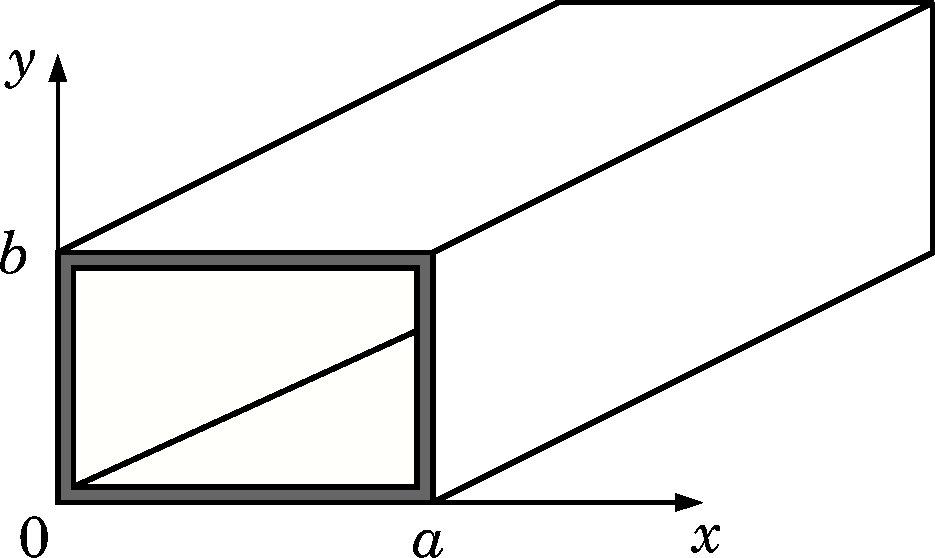
\includegraphics[width=0.4\textwidth]{guide_onde.pdf}
\end{figure}

On considère donc un guide d'onde métallique rectangulaire (largeur $a$, hauteur $h$) dans lequel se propage une onde élétromagnétique à la pulsation $\omega$. On suppose que le champ électrique s'écrit :
\begin{align*}
	\vec{E}=f(x,y)\cdot\exp[i(kz-\omega t)]\vec{e}_x
\end{align*}
Les parois sont de plus supposées infiniment conductrices et l'air à l'intérieur du guide est assimilé au vide. On souhaite comprendre les caractéristiques de la propagation dans le guide par rapport à celle dans le vide.

\begin{itemize}

	\item[$\bigstar$] A t-on affaire à une OPPM ? Justifier.
	
	\item[$\bigstar$] A partir des équations de Maxwell, montrer que $f$ ne dépend que de $x$ et retrouver l'équation de propagation vérifiée par $\vec{E}$. En déduire l'équation différentielle vérifiée par $f$ et montrer qu'il existe deux types de solution.
	
	\item[$\bigstar$]  A partir des conditions aux limites, montrer qu'il ne peut y avoir qu'un seul type de solution non nulle pour $\vec{E}$ et donner son expression. 
	
	\item[$\bigstar$] En déduire une inégalité sur la longueur d'onde $\lambda$, puis déterminer la relation de dispersion reliant $k$ et $\omega$. Pourquoi parle t-on de modes ou de quantification ? Pour une fréquence donnée, combien de modes peuvent se propager dans le guide ? Représenter $\vec{E}$ pour les deux premier modes à un instant donné.
	
	\item[$\bigstar$] Donner l'expression du champ magnétique $\vec{B}$. 
	
	\item[$\bigstar$] Calculer le vecteur de Poynting $\vec{\Pi}$ de l'onde. Commenter.
	
	\item[$\bigstar$] Estimer la norme de $\vec{\Pi}$ dans le cas d'un micro-onde domestique.

\end{itemize}

\newpage

\section*{Réflexion sur un conducteur de conductivité finie}

Un milieu conducteur de conductivité $\gamma=6\cdot10^7\Omega^{-1}$m$^{-1}$ occupe le demi-espace $z>0$ tandis que de l'air, assimilé au vide, occupe le demi-espace $z<0$. Une onde électromagnétique incidente plane et monochromatique de pulsation $\omega$ se propage dans la direction de l'axe $Oz$ dans l'air. Le champ électrique de cette onde incidente s'écrit :
\begin{align*}
	\vec{E}_i=\vec{E}_{0,i}\exp[i(\omega t-k_iz)]
\end{align*}
en notant $\vec{E}_{0,i}$ son amplitude.
A l'interface $z=0$, elle donne naissance à une onde réfléchie et une onde transmise s'écrivant respectivement $\vec{E}_r=\vec{E}_{0,r}\exp[i(\omega t+k_rz)]$ et $\vec{E}_t=\vec{E}_{0,t}\exp[i(\omega t-k_tz)]$, toutes de même pulsation $\omega$. On admet que les amplitudes des champs éléectriques appartiennent au plan $xOy$.

\begin{itemize}
	
	\item[$\clubsuit$] Déterminez l'équation de propagation vérifiée par le champ électrique dans le vide, et en déduire l'expression de $k_i$ et $k_r$ en fonction de $\omega$ et $c$, la vitesse de la lumière. 
	
	\item[$\clubsuit$] Quelle équation vérifie le champ électrique à l'intérieur du métal, pour des fréquences que l'on supposera ici inférieures au GHz ? En déduire l'expression de $k_t$. Commenter. 
	
	\item[$\clubsuit$] Déterminer l'expression du champ magnétique $\vec{B}_i$ en fonction de l'amplitude du champ électrique incident, $\vec{E}_{0,i}$, et des données de l'enoncé. Déterminer de la même manière $\vec{B}_r$ et $\vec{B}_t$ respectivement en fonction de $\vec{E}_{0,r}$ et $\vec{E}_{0,t}$.
	
	\item[$\clubsuit$] Quelles sont les conditions imposées aux champ électrique et magnétique à l'interface $z=0$ ? En déduire les coefficients de réflexion $r=E_{0,r}/E_{0,i}$ et de transmission $t=E_{0,t}/E_{0,i}$.
	
	\item[$\clubsuit$] Après avoir déterminé les moyennes temporelles des vecteurs de Poynting $\vec{Pi}$ des trois ondes	, déterminer le coefficient de réflexion $R$ et de transmission $T$ en énergie. Commenter.
	
	\item[$\clubsuit$] Quelle est la puissance moyenne dissipée par effet Joule dans le métal, par unité de surface. Donner une estimation dans le cas où cette plaque est exposée en plein soleil.
	
\end{itemize}

\end{document}